\chapter{闭卷条件下的声明级论证裁决方法与受控评测}\label{ch:clara}

本章研究\emph{闭卷}条件下的虚假新闻检测：只根据新闻文本本身判断真伪，不使用传播数据，也不检索外部证据。针对已有“LLM 提供理由、小模型裁决”一类方法中理由可用性判断粒度过粗、辩论类方法调用开销大这两个问题，本章提出声明级论证裁决方法 \method{}（Claim-Level Argument Reliability Adjudication）；同时设计了一套控制 LLM、超参数搜索与随机性的评测流程，以及分析替换、风格改写、单句事实篡改与留一领域四项受控测试。

需要预先说明的是，本章的实验结果并不都支持方法设计时的设想，我们如实报告：\method{} 在分布内与已有方法持平，其各个部件中只有相关性门控被证明有效；受控测试进一步表明，包括 LLM 自身判断在内的闭卷检测器主要依赖文风，而不是新闻内容是否属实。这些发现既是本章的结论，也是第~\ref{ch:openbook}~章转向证据驱动验证的直接动机。

本章的安排如下：\ref{sec:problem}~节给出问题定义；\ref{sec:method}~节介绍 \method{} 的结构与训练方法；\ref{sec:setup}~节说明数据集、对比方法与评测协议；\ref{sec:results}~节报告并分析实验结果；\ref{sec:discussion}~节讨论这些结果的含义与局限；\ref{sec:ch3-summary}~节小结。

\section{问题定义}\label{sec:problem}

给定一条新闻或社交媒体消息 $x$（仅文本），闭卷虚假新闻检测要求在\textbf{不检索任何外部证据}的条件下预测其真实性标签 $y\in\{0,1\}$（$1$ 表示虚假）。训练集 $\mathcal{D}=\{(x_i,y_i)\}$ 只含新闻级标签。除新闻级概率 $\hat y=P(y{=}1\mid x)$ 外，我们还希望模型（i）给出新闻中各条声明存在问题的概率，用于定位；（ii）能够判断 LLM 给出的每个分析单元是否可用，并在不可用时退回到只依赖新闻文本的判断。

本文把 $x$ 视为一个由若干\emph{实例}组成的包（bag），沿用多示例学习（multiple instance learning, MIL）的标准假设\citep{dietterich1997solving,carbonneau2018mil}：记隐变量 $z_k\in\{0,1\}$ 表示第 $k$ 个实例是否存在问题，则
\begin{equation}
y=1 \iff \exists k,\ z_k=1 .\label{eq:mil}
\end{equation}
该假设蕴含一个不对称性：真新闻（$y{=}0$）的所有实例都满足 $z_k{=}0$，而假新闻（$y{=}1$）只保证至少一个实例有问题。假设何时不成立见 \ref{sec:discussion}~节的讨论。

\section{\method{} 方法}\label{sec:method}

\subsection{总体框架}

\method{}（\textbf{C}laim-\textbf{L}evel \textbf{A}rgument \textbf{R}eliability \textbf{A}djudication）由一个冻结的 LLM 与一个可训练的小模型裁决器组成（图~\ref{fig:framework}）。LLM 把新闻分解为若干声明，并为每条声明写出正反两方论证；裁决器读取新闻原文与 LLM 的输出，逐个实例决定是否采用、采用多少，再聚合为新闻级判定。LLM 的输出离线生成并缓存，训练与推理阶段裁决器不再访问 LLM。

\begin{figure}[htbp]
\centering
\resizebox{\linewidth}{!}{% Framework figure (TikZ); natural width ~172 mm, scaled to \linewidth where it is included.
% Orange = LLM-side quantities, blue = SLM-side, green = gates.
\definecolor{cLLM}{HTML}{EB6834}
\definecolor{cSLM}{HTML}{2A78D6}
\definecolor{cGate}{HTML}{1BAF7A}
\definecolor{cInk}{HTML}{0B0B0B}
\definecolor{cMuted}{HTML}{6B6A66}
\definecolor{cLine}{HTML}{C3C2B7}
\begin{tikzpicture}[
  x=1mm, y=1mm, font=\footnotesize, >={Stealth[length=1.6mm]},
  box/.style={draw=cLine, rounded corners=2pt, fill=white, align=center, inner sep=2.5pt, text=cInk},
  llm/.style={box, draw=cLLM!80, fill=cLLM!7},
  slm/.style={box, draw=cSLM!80, fill=cSLM!7},
  gate/.style={box, draw=cGate!90, fill=cGate!9},
  flow/.style={->, draw=cMuted, line width=0.5pt},
  sup/.style={->, draw=cMuted, dashed, line width=0.5pt},
  lab/.style={font=\scriptsize, text=cMuted, inner sep=1.5pt}]

% ---------------- column A: news and LLM
\node[box, minimum width=31mm] (x) at (0,0) {新闻 $x$\\[-1pt]{\scriptsize 句子 $s_1,\dots,s_n$}};
\node[llm, minimum width=31mm] (llm) at (0,-19) {冻结的 LLM\\[-1pt]{\scriptsize 离线生成，结构化解码}};
\node[llm, minimum width=31mm, align=left] (out) at (0,-40.5) {%
  {\scriptsize 声明 $c_k$（类型 $t_k$，句 $j_k$）}\\[-1pt]
  {\scriptsize 论证 $a_k^{+},a_k^{-}$，怀疑度 $v_k$}\\[-1pt]
  {\scriptsize 整体判断（$k=0$）}\\[-1pt]
  {\scriptsize 论证前评分 $\tilde v_0$}};
\draw[flow] (x) -- (llm);
\draw[flow] (llm) -- (out);

% ---------------- column B: evidence and gates
\node[slm, minimum width=45mm] (sx) at (47,0) {整体文本分支\\[-1pt]{\scriptsize $s_x=\mathrm{MLP}_x(\bm h_x)$}};
\node[slm, minimum width=45mm] (sslm) at (47,-19) {SLM 证据\\[-1pt]{\scriptsize $s_k^{\mathrm{slm}}=\mathrm{MLP}_s(\bm c_k)$}};
\node[llm, minimum width=45mm] (sllm) at (47,-31.5) {LLM 证据\\[-1pt]{\scriptsize $s_k^{\mathrm{llm}}=\mathrm{MLP}_a(\Delta\bm u_k)+\alpha\,\mathrm{logit}\,v_k$}};
\node[gate, minimum width=45mm] (g) at (47,-44) {判定门控\\[-1pt]{\scriptsize $g_k$：LLM 证据的权重}};
\node[gate, minimum width=45mm] (r) at (47,-56.5) {相关性门控\\[-1pt]{\scriptsize $r_k$：该实例是否属于这条新闻}};

% ---------------- columns C, D: combination
\node[box, minimum width=40mm] (pk) at (97,-37.75) {实例概率\\[-1pt]{\scriptsize $p_k=\sigma\big(b_0+r_k(s_k^{\mathrm{slm}}+g_k\,s_k^{\mathrm{llm}})\big)$}\\[-1pt]{\scriptsize $r_k\to0$：空实例，$p_k\to\sigma(b_0)$}};
\node[box, minimum width=41mm] (nor) at (143,-37.75) {noisy-OR 聚合\\[-1pt]{\scriptsize $P_{\mathrm{MIL}}=1-\prod_k(1-p_k)$}};
\node[box, minimum width=41mm] (y) at (143,0) {新闻级预测\\[-1pt]{\scriptsize $\hat y=\sigma\big(s_x+\tilde\gamma\,[\mathrm{logit}\,P_{\mathrm{MIL}}-\mathrm{logit}\,P_{\varnothing}]+b\big)$}};

% ---------------- flows
\draw[flow] (x) -- (sx);
\coordinate (bus) at (20,-40.5);
\draw[draw=cMuted, line width=0.5pt] (out.east) -- (bus);
\draw[flow] (bus) |- (sslm.west);
\draw[flow] (bus) |- (sllm.west);
\draw[flow] (bus) |- (g.west);
\draw[flow] (bus) |- (r.west);
\coordinate (join) at (73,-37.75);
\draw[draw=cMuted, line width=0.5pt] (sslm.east) -| (join);
\draw[draw=cMuted, line width=0.5pt] (sllm.east) -| (join);
\draw[draw=cMuted, line width=0.5pt] (g.east) -| (join);
\draw[draw=cMuted, line width=0.5pt] (r.east) -| (join);
\draw[flow] (join) -- (pk.west);
\draw[flow] (pk) -- (nor);
\draw[flow] (nor) -- (y);
\draw[flow] (sx) -- (y);

% ---------------- instance plate
\begin{scope}[on background layer]
  \node[draw=cLine, dashed, rounded corners=3pt, inner sep=3pt, fit=(sslm)(sllm)(g)(r)(pk)] (plate) {};
\end{scope}
\node[lab, anchor=south east] at ([xshift=-1mm,yshift=0.5mm]plate.south east) {对每个实例 $k=0,\dots,K$};

% ---------------- supervision (training only)
\node[lab] (lcls) at (143,11) {$\mathrm{BCE}(\hat y,\,y)$};
\node[lab] (lmil) at (143,-50) {$\mathrm{BCE}(P_{\mathrm{MIL}},\,y)$};
\node[lab, align=left] (lgate) at (97,-54) {$\mathcal L_{\mathrm{gate}}$：LLM 是否站对边\\[-1pt]$\mathcal L_{\mathrm{rel}}$：错配负例};
\draw[sup] (lcls) -- (y);
\draw[sup] (lmil) -- (nor);
\draw[sup] (lgate.west) -- ++(-6,0) |- ([yshift=-2mm]g.east);
\draw[sup] (lgate.west) -- ++(-6,0) |- ([yshift=-2mm]r.east);
\end{tikzpicture}
}
\caption{\method{} 总体框架}\label{fig:framework}
\note{LLM 产生整体实例（$k{=}0$）与 $K$ 条声明，每个实例附带支持论证 $a^+$、质疑论证 $a^-$ 与怀疑度 $v$。裁决器对每个实例计算 SLM 证据、LLM 证据、判定门控 $g$ 与相关性门控 $r$；$r\to0$ 的实例成为不携带证据的空实例。实例经 noisy-OR 聚合后，以“全为空实例的包”为基准与整体文本分支融合。$\Delta\bm u_k$ 表示两方论证表示的差与逐元素积，$\tilde\gamma=\softplus(\gamma)$。虚线表示只在训练时使用的监督信号。}
\end{figure}

\subsection{声明分解与双立场论证}\label{sec:llm}

\subsubsection{输出结构}
先用确定性规则把 $x$ 切分为句子 $s_1,\dots,s_n$（$n\le 12$）并编号。LLM 读取编号后的文本，在一次调用中按固定顺序生成一个 JSON 对象：
\begin{enumerate}
\item \textbf{第一印象} $v^{\mathrm{fi}}$：在做任何分析之前，对“整条消息是虚假或误导性信息”的 1--5 级评分；
\item \textbf{声明列表} $\{c_k\}_{k=1}^{K}$（$K\le 6$）：每条声明包含自包含的声明文本、类型 $t_k\in\{$事实、数字、引述、观点$\}$、所在句子编号 $j_k$、认为其可信的最强理由 $a_k^+$、认为其可疑的最强理由 $a_k^-$，以及 1--5 级怀疑度；
\item \textbf{整体判断}：对整条消息的正反理由 $a_0^+,a_0^-$ 与 1--5 级怀疑度。
\end{enumerate}
整体判断在裁决器中作为第 $0$ 个实例，用于覆盖标题与正文不符、来源不明、情绪煽动等无法归到单条声明上的问题。完整提示词见附录~\ref{app:prompt}。

\subsubsection{设计动机}
与多轮辩论\citep{liu2025ted,han2025d2d}相比，这一设计有三点考虑。其一，把论证单位从“发言轮次”换成“声明”，每个声明都有成对的正反论证，裁决器可以直接比较两方，调用次数不随论证数量增长。其二，要求 LLM 先写两方论证、最后才给评分，并禁止在论证中写结论，以减轻先下结论再找理由的立场锁定。其三，提示词要求保留归属（“某人称……”不得改写为既成事实），因为一条真新闻可以如实转述一个不实说法，丢掉归属会直接破坏式~\eqref{eq:mil} 的假设。

\subsubsection{结构化解码与软评分}
生成时用 JSON schema 约束解码\citep{kwon2023vllm,dong2024xgrammar}：声明数下限随句子数增加（$n\le2$ 时为 1，$n\le4$ 时为 2，否则为 3），句子编号限制在 $\{1,\dots,n\}$ 内。评分不直接使用生成的整数，而是取评分位置上五个等级 token 的概率 $\pi_\ell$ 并归一化，计算期望
\begin{equation}
v=\sum_{\ell=1}^{5}\frac{\ell-1}{4}\,\pi_\ell\in[0,1],
\end{equation}
同时保留归一化熵 $H(\pi)$ 作为 LLM 自身不确定性的度量。为避免评分受最后写下的论证影响，我们按样本编号的奇偶确定性地交替 $a^+$ 与 $a^-$ 的书写顺序，使这一潜在偏置与标签无关。

\subsubsection{论证前的整体评分}
整体实例除论证后的怀疑度 $v_0$ 外，还带有一个论证前的评分 $\tilde v_0$。默认取 LLM 对同一条消息的零样本判断概率 $p_{\mathrm{zs}}$：它来自一次只输出一个 token 的额外调用，取“0”“1”两个 token 的归一化概率。在从训练集抽取的开发样本上，$p_{\mathrm{zs}}$ 的区分度不低于提示内的第一印象 $v^{\mathrm{fi}}$。若要求严格的单次调用，可令 $\tilde v_0=v^{\mathrm{fi}}$，这一变体在消融实验中报告。

\subsection{编码}\label{sec:enc}

所有方法遵循 ARG\citep{hu2024bad} 的设置：预训练编码器只微调最后一层，其余层冻结。\method{} 使用两份最后一层的可训练副本，$E_x$ 编码新闻原文，$E_a$ 编码 LLM 侧文本。记 $\operatorname{Pool}$ 为可学习的注意力池化，则
\begin{align}
\bm H_x &= E_x(x), & \bm h_x &= \operatorname{Pool}(\bm H_x),\\
\bm c_k &= \operatorname{Pool}\!\big(E_a(c_k)\big), & \bm u_k^{\pm} &= \operatorname{Pool}\!\big(E_a([c_k;a_k^{\pm}])\big),\\
\bm e_k &= \operatorname{LN}\!\big(\bm c_k+\operatorname{CrossAttn}(\bm c_k,\bm H_x)\big),
\end{align}
其中 $[c_k;a_k^{\pm}]$ 表示把声明与论证作为句对输入，$\bm e_k$ 是声明以自身为查询、对新闻 token 做交叉注意力后得到的上下文化表示。整体实例（$k{=}0$）的声明文本取一个固定短语。

由于冻结层的输出与训练轮次无关，我们对每条序列只做一次冻结层前向并缓存其隐状态，训练时仅计算最后一层。这与每步重新计算有三点差别：冻结层没有 dropout 噪声，缓存的隐状态以半精度存储，可训练的层用混合精度计算。附录~\ref{app:live} 核对了它们对结果的影响。

\subsection{实例证据}\label{sec:score}

对每个实例计算两路证据：
\begin{align}
s_k^{\mathrm{slm}} &= \operatorname{MLP}_s(\bm c_k),\\
s_k^{\mathrm{llm}} &= \operatorname{MLP}_a\!\big([\bm u_k^- - \bm u_k^+;\ \bm u_k^-\odot\bm u_k^+]\big)+\alpha\,\logit(v_k)+\mathbf{1}[k{=}0]\,\alpha_0\,\logit(\tilde v_0),
\end{align}
其中 $\alpha,\alpha_0$ 为可学习标量。$s^{\mathrm{llm}}$ 中的差分与逐元素积显式刻画两方论证的不对称，即“哪一方更容易被辩护”。

两路证据都只依赖该实例自身的输入：声明文本、它的两条论证与评分，而不依赖新闻整体表示 $\bm h_x$。这是有意为之。若实例证据可以看到整条新闻，noisy-OR 型 MIL 存在一个平凡解：每个实例都输出新闻级判断的副本。此时新闻级精度不受影响，但实例概率失去实例含义，定位无从谈起。新闻级的文本证据另有通道（\ref{sec:agg} 节的 $s_x$）。实验中我们把允许实例证据读取 $\bm e_k$ 与 $\bm h_x$ 的耦合变体作为消融对照。

\subsection{相关性门控、判定门控与空实例}\label{sec:gate}

LLM 的输出在两个层面上可能不可用。第一，分析单元本身可能不是这条新闻的忠实分析：声明可能是幻觉出来的，或者整份分析与新闻对不上。第二，即使声明忠实于原文，LLM 对它的判断也可能是错的。\method{} 用两个门控分别处理：
\begin{align}
r_k&=\sigma\!\Big(\operatorname{MLP}_r\big([\bm e_k;\ \bm h_x;\ \bm c_k\odot\bm h_x;\ |\bm c_k-\bm h_x|;\ \bar{\bm u}_k\odot\bm h_x;\ |\bar{\bm u}_k-\bm h_x|]\big)\Big),\label{eq:rk}\\
g_k&=\sigma\!\Big(\operatorname{MLP}_g\big([\bm e_k;\ \bm h_x;\ \bm u_k^+;\ \bm u_k^-;\ \operatorname{emb}(t_k);\ \bm\phi_k]\big)\Big),\label{eq:gk}
\end{align}
其中 $\bar{\bm u}_k=\tfrac12(\bm u_k^++\bm u_k^-)$，$\bm\phi_k=[v_k,\ |v_k-0.5|,\ \tilde v_k,\ |\tilde v_k-v_k|,\ H(\pi_k)]$ 是由评分导出的特征（声明取 $\tilde v_k=v_k$）。\emph{相关性门控} $r_k$ 通过声明、论证与新闻表示之间的匹配特征判断该实例是否属于这条新闻；\emph{判定门控} $g_k$ 调节 LLM 证据的权重。实例存在问题的概率为
\begin{equation}
p_k=\sigma\!\Big(b_0+r_k\big(s_k^{\mathrm{slm}}+g_k\,s_k^{\mathrm{llm}}\big)\Big),\label{eq:pk}
\end{equation}
其中 $b_0$ 是可学习的标量。当 $r_k\to0$ 时，$p_k\to\sigma(b_0)$，与实例内容无关：该实例退化为一个只携带先验的\emph{空实例}。LLM 输出无法解析的新闻，其实例直接取 $r_k=0$。

\subsection{Noisy-OR 聚合与以空包为基准的融合}\label{sec:agg}

在实例相互独立的近似下，式~\eqref{eq:mil} 对应 noisy-OR 聚合\citep{maron1998framework}：
\begin{equation}
P_{\mathrm{MIL}}=1-\prod_{k=0}^{K}(1-p_k).
\end{equation}
新闻原文的整体表示在已有工作中贡献最大\citep{he2026factguard}，因此保留一个整体文本分支 $s_x=\operatorname{MLP}_x(\bm h_x)$。两者的融合以“全部为空实例的包”为基准：
\begin{equation}
\hat y=\sigma\!\Big(s_x+\softplus(\gamma)\cdot\big[\logit(P_{\mathrm{MIL}})-\logit(P_{\varnothing})\big]+b\Big),\qquad
P_{\varnothing}=1-\big(1-\sigma(b_0)\big)^{K+1},\label{eq:fuse}
\end{equation}
其中 $\gamma,b$ 为可学习标量。方括号内是实例提供的、相对于“没有任何可用实例”的证据。它有两个作用。其一，当所有实例都是空实例时该项恰为 $0$，预测精确地退回到文本分支 $\sigma(s_x+b)$。其二，$P_{\varnothing}$ 随实例数变化，抵消了 noisy-OR“实例越多概率越高”的长度偏置。

\subsection{训练目标}\label{sec:loss}

总损失为
\begin{equation}
\mathcal L=\operatorname{BCE}(\hat y,y)+\lambda_{\mathrm{mil}}\operatorname{BCE}(P_{\mathrm{MIL}},y)+\lambda_{\mathrm{rel}}\,\mathcal L_{\mathrm{rel}}+\lambda_{\mathrm{gate}}\,\mathcal L_{\mathrm{gate}} .
\end{equation}
当 $y{=}0$ 时，$\operatorname{BCE}(P_{\mathrm{MIL}},0)=-\sum_k\log(1-p_k)$，即对真新闻的每个实例施加了精确的负监督，这是 MIL 不对称性带来的实例级监督。

\subsubsection{错配负例与相关性损失}
现有数据中，每条新闻的 LLM 分析都是针对它自己生成的，模型没有机会学习“这份分析不属于这条新闻”。我们在训练时构造\emph{错配负例}：每个小批量中，每条新闻以概率 $\rho$ 被换上同一批内另一条新闻的全部 LLM 分析。被替换的新闻保留自己的标签，它的所有实例以 $r_k=0$ 为相关性目标，其余实例以 $r_k=1$ 为目标：
\begin{equation}
\mathcal L_{\mathrm{rel}}=\overline{\operatorname{BCE}}\big(r_k,\ \mathbf{1}[\text{实例 }k\text{ 属于该新闻}]\big).
\end{equation}
被替换的新闻不参与 $\operatorname{BCE}(P_{\mathrm{MIL}},y)$ 与 $\mathcal L_{\mathrm{gate}}$，但参与 $\operatorname{BCE}(\hat y,y)$。由于此时实例被学成空实例，式~\eqref{eq:fuse} 中只剩文本分支，裁决器因此同时学到了在分析不可用时仅凭文本做判断。

\subsubsection{判定门控的弱监督}
判定门控的监督目标是“LLM 在该实例上是否站对了边”。记 LLM 的表态分数为 $\bar v_k$（整体实例取 $(v_0+\tilde v_0)/2$，声明取 $v_k$），$\bar v_k>0.5+\delta$ 视为判其有问题，$\bar v_k<0.5-\delta$ 视为判其无问题，介于两者之间视为未表态，不参与该项损失。目标为
\begin{equation}
q_k=\hat z_k\cdot\mathbf{1}[\bar v_k>0.5+\delta]+(1-\hat z_k)\cdot\mathbf{1}[\bar v_k<0.5-\delta],
\end{equation}
其中 $\hat z_k$ 是对隐状态 $z_k$ 的估计：整体实例取 $\hat z_0=y$；真新闻中的声明由 MIL 不对称性取 $\hat z_k=0$；假新闻中的声明取 noisy-OR 后验 $\hat z_k=\sg[p_k/P_{\mathrm{MIL}}]$（$\sg$ 表示停止梯度），在 $T_w$ 轮 warm-up 之后启用并以权重 $\eta$ 计入。$\mathcal L_{\mathrm{gate}}$ 是 $\operatorname{BCE}(g_k,q_k)$ 在已表态实例上的加权平均。需要说明的是，这一监督信号很弱，判定门控实际学到了什么需要用实验检验，见 \ref{sec:exp-gate} 节。

算法~\ref{alg:train} 给出完整的训练流程。

\begin{algorithm}[t]
\caption{\method{} 的训练}\label{alg:train}
\KwIn{训练集 $\mathcal D$；冻结的 LLM；超参数 $\lambda_{\mathrm{mil}},\lambda_{\mathrm{rel}},\lambda_{\mathrm{gate}},\rho,\eta,\delta,T_w$}
\KwOut{裁决器参数 $\theta$}
\ForEach{$x\in\mathcal D_{\mathrm{train}}\cup\mathcal D_{\mathrm{val}}\cup\mathcal D_{\mathrm{test}}$}{
  $A(x)\leftarrow\operatorname{LLM}(x)$\tcp*{离线生成并缓存}
}
缓存所有序列的冻结层隐状态\;
\For{$\mathrm{epoch}=0,1,\dots$}{
  \ForEach{小批量 $\{(x_i,y_i,A_i)\}$}{
    以概率 $\rho$ 把 $A_i$ 替换为批内另一条新闻的分析，记 $m_i=1$（否则 $m_i=0$）\;
    计算 $\bm h_x,\bm c_k,\bm e_k,\bm u_k^\pm$，以及 $s_k^{\mathrm{slm}},s_k^{\mathrm{llm}},r_k,g_k,p_k$\;
    $P_{\mathrm{MIL}}\leftarrow1-\prod_k(1-p_k)$；按式~\eqref{eq:fuse} 计算 $\hat y$\;
    $\mathcal L\leftarrow\operatorname{BCE}(\hat y,y)+\lambda_{\mathrm{rel}}\overline{\operatorname{BCE}}(r_k,1-m)$\;
    对 $m_i=0$ 的新闻：$\mathcal L\mathrel{+}=\lambda_{\mathrm{mil}}\operatorname{BCE}(P_{\mathrm{MIL}},y)+\lambda_{\mathrm{gate}}\mathcal L_{\mathrm{gate}}$（$\mathrm{epoch}<T_w$ 时不含假新闻声明）\;
    更新 $\theta$\;
  }
  在验证集上计算 macro-F1，按早停规则保留最优参数\;
}
\end{algorithm}

\subsection{\student{}：声明到句子对齐的蒸馏}\label{sec:student}

为了在推理时完全不调用 LLM，我们训练一个只读新闻的学生模型。学生以新闻的\emph{句子}为 MIL 实例（外加一个整体实例），沿用教师的 SLM 证据分支：$p_j^S=\sigma\big(b_0+\operatorname{MLP}_s(\bm c_j)\big)$，聚合与融合方式同式~\eqref{eq:fuse}。LLM 为每条声明给出的句子编号 $j_k$ 把教师的声明级概率对齐到句子：
\begin{equation}
t_j=\max_{k:\,j_k=j}p_k^{T},
\end{equation}
没有声明与之对齐的句子不参与实例级蒸馏。学生的损失为
\begin{equation}
\begin{aligned}
\mathcal L_S={}&\operatorname{BCE}(\hat y^S,y)+\lambda_{\mathrm{mil}}\operatorname{BCE}(P^S_{\mathrm{MIL}},y)\\
&+\kappa_{o}\operatorname{BCE}(\hat y^S,\hat y^T)+\kappa_{i}\,\overline{\operatorname{BCE}}(p^S_j,t_j)+\kappa_{f}\operatorname{MSE}(\bm h^S_x,\bm h^T_x),
\end{aligned}
\end{equation}
参数由教师的对应模块初始化。ARG-D 与 FactGuard-D 只蒸馏池化后的特征向量，学生没有实例级输出；\student{} 的学生保留了句级输出。

\subsection{选择性预测}\label{sec:selective}

闭卷条件下部分新闻无法从内容判定。除常用的 MaxProb 置信度 $|\hat y-0.5|$ 外，我们在验证集上拟合一个逻辑回归选择器，预测裁决器自身的判定是否正确，输入特征为 $|\hat y-0.5|$、两分支分歧 $|P_{\mathrm{MIL}}-\sigma(s_x)|$、判定门控均值、$\max_k p_k$、$|P_{\mathrm{MIL}}-0.5|$ 与实例数的对数。选择器不接触测试标签。

\subsection{开销}\label{sec:cost}

默认配置下每条新闻需要一次结构化调用与一次只输出一个 token 的零样本调用。裁决器在 BERT-base 规模的编码器上增加一份最后一层副本与若干 MLP。每条新闻需要编码 $1+3(K{+}1)$ 条短序列（新闻、每个实例的声明及两个声明--论证对），其冻结层前向只做一次。实测开销见 \ref{sec:exp-cost} 节。

\section{实验设置}\label{sec:setup}

\subsection{数据集}

实验使用 ARG\citep{hu2024bad} 发布的两个按时间划分的数据集：中文的 Weibo21\citep{nan2021mdfend} 与英文的 GossipCop\citep{shu2020fakenewsnet}。训练集早于验证集与测试集，更接近真实部署中“用过去的数据检测未来的新闻”的情形。统计信息见表~\ref{tab:data}。两个数据集的类别分布不同：Weibo21 大致均衡，GossipCop 的假新闻不足五分之一，因此以 macro-F1 为主指标。

\begin{table}[htbp]
\centering\small
\caption{数据集统计}\label{tab:data}
\fittable{gen/tables/data.tex}
\note{声明数为 Qwen2.5-7B 对每条新闻分解出的声明条数（不含整体实例）。}
\end{table}

\subsection{对比方法}

所有需要 LLM 的方法使用同一个 LLM，即 Qwen2.5-7B-Instruct\citep{qwen25}，以排除“换了更强的 LLM”这一混淆因素。

\begin{itemize}
\item \textbf{仅 LLM（不训练）}：零样本与零样本 CoT\citep{kojima2022large} 判断，提示词沿用 ARG。作为参照，同时列出 ARG 数据中附带的 GPT-3.5 判断。
\item \textbf{BERT}\citep{devlin2019bert}：只读新闻文本的 SLM 基线。
\item \textbf{LoRA-LLM}：用 LoRA\citep{hu2022lora} 把 Qwen2.5-7B 直接微调为分类器。模型读取与零样本基线完全相同的提示，在答案位置对“0”“1”两个 token 的 logit 做二分类交叉熵，因此它与零样本基线的差别只在于微调。
\item \textbf{BERT+ZS}：在 BERT 的输出 logit 上加一项 $w\cdot\logit(p_{\mathrm{zs}})$，$p_{\mathrm{zs}}$ 是 LLM 零样本判断为假的概率，$w$ 为可学习标量。这是利用 LLM 的最简单方式，用来衡量更复杂的协同结构在此之上还能带来多少。
\item \textbf{ARG}\citep{hu2024bad} 与 \textbf{FactGuard}\citep{he2026factguard}：按官方代码重新实现了前向计算与损失。ARG 的两条理由、FactGuard 的 topic-content 与常识理由均用官方提示词由 Qwen2.5-7B 重新生成（与官方流程的差异见附录~\ref{app:impl}）。对 ARG 另外报告使用数据集自带 GPT-3.5 理由的结果，以便与原论文对照。
\item \textbf{学生模型}：ARG-D、FactGuard-D 与 \student{}，推理时不调用 LLM。
\end{itemize}
TED\citep{liu2025ted} 的官方仓库在本文写作时尚未放出代码，D2D\citep{han2025d2d} 依赖 GPT-4o，两者未能在相同条件下复现，故不列入对比。

\subsection{训练与评测协议}\label{sec:protocol}

所有基于 SLM 的方法共用 ARG 官方实现的协议：编码器只微调最后一层；批大小 64；最多 50 轮；按验证集 macro-F1 早停（耐心值 5）；判定阈值固定为 0.5；测试集只在选定的检查点上评估一次。编码器统一为 chinese-bert-wwm-ext\citep{cui2021wwm}（中文）与 bert-base-uncased（英文）。在此基础上我们做了三点统一，以保证比较公平：
\begin{enumerate}
\item \textbf{多种子}：主实验每个配置运行 5 个随机种子，报告均值与标准差；LoRA-LLM、蒸馏、留一领域、敏感性实验以及英文上的消融实验为 3 个种子。
\item \textbf{相同的学习率搜索}：每个方法都在 $\{2\times10^{-5},5\times10^{-5}\}$ 上运行（即 ARG 与 FactGuard 官方配置在两个数据集上使用的两个值），按种子平均的验证集 macro-F1 选择。全部网格点的结果见附录表~\ref{tab:grid}。
\item \textbf{基线超参数}：ARG 与 FactGuard 的损失权重取自各自官方脚本。
\end{enumerate}

为了在单张显卡上完成全部多种子实验，各 SLM 类方法训练时缓存冻结编码器层的输出，可训练的层使用混合精度；附录~\ref{app:live} 在全精度下复核了主实验，定性结论不变。

\method{} 的损失权重等超参数为预先设定的固定值，没有做搜索：$\lambda_{\mathrm{mil}}{=}0.5$，$\lambda_{\mathrm{rel}}{=}0.5$，$\lambda_{\mathrm{gate}}{=}0.3$，错配负例比例 $\rho{=}0.2$，$\eta{=}0.5$，$\delta{=}0.05$，$T_w{=}2$，$K\le6$，$b_0$ 初始化为 $-2$；敏感性分析见附录~\ref{app:sens}。所有模块与基线一样使用同一个学习率。

\subsubsection{关于开发过程的说明}
提示词在从训练集抽取的 400 条样本上调试。\method{} 经历过一次结构修改：最初的版本没有相关性门控，它在 Weibo21 上的一轮完整实验（包括测试集）显示，把 LLM 分析替换为其他新闻的分析会使其性能大幅下降。相关性门控、空实例与错配负例是针对这一问题加入的，此后的结构选择（是否为新模块使用更大的学习率、判定门控的几种替代形式）只依据验证集上的诊断做出，未再参考测试集。最初的版本与消融实验中“去掉相关性门控与错配负例”一行基本对应（两者在融合的基准项上还有细小差别）。本章报告的全部结果来自修改后重新运行的实验。

\subsubsection{显著性检验}
我们报告两种检验。（i）对测试样本的配对 bootstrap\citep{koehn2004statistical}（5{,}000 次重采样，统计量为种子平均的 macro-F1 之差），记其 $p$ 值为 $p_{\text{样本}}$；它刻画测试集有限带来的不确定性，但把已训练好的模型视为固定。（ii）对随机种子的 Welch $t$ 检验，记为 $p_{\text{种子}}$；它刻画训练的随机性，在种子数较少时功效有限。只有两者都在 0.05 水平上成立时，本文才称一个差异显著；所有检验均未做多重比较校正。

\subsection{分布内精度之外的评测}\label{sec:robust-sets}

\subsubsection{LLM 分析不可用}
我们用两种粒度的替换模拟 LLM 给出与新闻不符的分析，新闻原文与标签始终不变。\emph{整条替换}：把测试集中比例为 $\rho'$ 的样本的全部 LLM 输出（包括零样本评分）替换为另一条随机测试样本的输出，模拟分析与新闻完全对不上的情形。\emph{单元替换}：对每条样本，以概率 $\rho'$ 把分析中的每个单元独立地替换为其他样本的单元，模拟部分幻觉；对 \method{}，单元是一条声明及其论证与评分，对 ARG 与 FactGuard，单元是自由文本理由（及 topic-content）中的一个句子。不由这类单元构成的整体判断与零样本评分保持不变。一个知道哪些分析不该采信的检测器，性能应平缓地退回到仅文本的水平。作为对照，我们还给 ARG 加上与 \method{} 相同的错配负例训练（记为 ARG+错配负例）：被替换理由的可用性目标置 0，新闻保留自己的标签。

\subsubsection{风格改写}
沿用 SheepDog\citep{wu2024sheepdog} 的风格攻击设定：把测试集中的假新闻改写为官方通稿文风，把真新闻改写为营销号文风，要求保留全部事实。改写由 Qwen3-8B\citep{qwen3} 完成，与负责分析的 Qwen2.5-7B 是不同的模型，避免同一模型既制造扰动又检测扰动；改写后的文本由 Qwen2.5-7B 重新分析。长度变化过大的改写被丢弃，结果只在成功改写的样本上统计，并与同一批样本的原文结果配对比较。

\subsubsection{定位：单句事实篡改}
现有数据集没有句级标注。为了定量评估定位能力，我们从测试集的真新闻中随机选一句，由 Qwen3-8B 提出一处最小的片段替换（否定、数字、时间、实体或结果），程序执行替换并校验替换确实改变了文字内容。得到的样本标签为假，且虚假信息的位置已知。评测指标为被篡改句子在模型给出的句子排序中的 Hit@1 与 MRR，并列时按随机打破的期望计算。黑盒分类器用遮挡归因\citep{li2016understanding}作为对照：逐句删除后预测为假的概率下降最多的句子即为其定位结果。需要强调，这是一个受控的合成基准，篡改后的句子未必在现实中为假，它衡量的是模型对局部事实改动的敏感位置是否正确。

\subsubsection{未见领域}
ARG 版本的 Weibo21 不含领域标签。我们用文本匹配从 Weibo21 原始发布中恢复了 83.5\% 样本的九类领域标签，并对测试样本不少于 100 条的六个领域做留一领域实验：训练集与验证集去掉该领域的全部样本，以及未能恢复领域标签的样本（它们可能属于被留出的领域），测试集只保留该领域的样本。各方法使用在完整数据上按验证集选出的学习率。

\subsubsection{拒答}
用风险--覆盖率曲线下面积（AURC）\citep{geifman2019bias}与固定覆盖率下的准确率评估选择性预测。

\section{实验结果与分析}\label{sec:results}

\subsection{分布内检测}\label{sec:main-results}

表~\ref{tab:main} 给出两个数据集上的主结果。

\begin{table}[htbp]
\centering\footnotesize
\setlength{\tabcolsep}{3.2pt}
\caption{两个数据集上的测试集结果（\%）}\label{tab:main}
\fittable{gen/tables/main.tex}
\note{可训练方法为多个随机种子的均值，下标为标准差（LoRA-LLM 与学生模型为 3 个种子，其余为 5 个）；每列最优的可训练方法加粗。$^\dagger$ 使用 ARG 数据自带的 GPT-3.5 输出，其余 LLM 输出均来自 Qwen2.5-7B。}
\end{table}

\subsubsection{\method{} 与已有的 LLM+SLM 方法持平，没有稳定的优势}
在 Weibo21 上 \method{} 的 macro-F1 为 \ptwo{CN/main/clara/macf1}，与 ARG（\ptwo{CN/main/arg/macf1}）几乎相同，高于 FactGuard（\ptwo{CN/main/factguard/macf1}）与 BERT（\ptwo{CN/main/bert/macf1}）约 1 个点。在 GossipCop 上 \method{} 为 \ptwo{EN/main/clara/macf1}，在 SLM 类方法中最高，比 ARG 高 \ptwo{EN/significance/arg/diff_mean} 个点。附录表~\ref{tab:sig} 给出两种检验的结果。在两个数据集上与 BERT、BERT+ZS、ARG（两种理由来源）和 FactGuard 的共十组比较中，按 \ref{sec:protocol} 节的标准只有 Weibo21 上对 FactGuard 的一组成立（$p_{\text{样本}}\peq{CN/significance/factguard/bootstrap/p}$，$p_{\text{种子}}\peq{CN/significance/factguard/welch_p}$），而且两个 $p$ 值都贴近 0.05、未做多重比较校正，证据很弱。在不使用混合精度的复核中（附录~\ref{app:live}），这一组不再成立（$p_{\text{样本}}\peq{CN/fp32/clara_vs/factguard/bootstrap/p}$，$p_{\text{种子}}\peq{CN/fp32/clara_vs/factguard/welch_p}$），成立的变成了 GossipCop 上对 FactGuard 的一组；对 BERT、BERT+ZS 与 ARG 的各组在两种精度下都不显著。对 BERT 的提升在 Weibo21 上只有对种子的检验成立（$p_{\text{种子}}\peq{CN/significance/bert/welch_p}$，$p_{\text{样本}}\peq{CN/significance/bert/bootstrap/p}$），在 GossipCop 上两者都不成立（\fthree{EN/significance/bert/welch_p} 与 \fthree{EN/significance/bert/bootstrap/p}）。分布内精度不是 \method{} 的优势所在。

\subsubsection{最简单的融合方式同样有效}
BERT+ZS 只在 BERT 的输出上加了一项 LLM 零样本评分，在 Weibo21 上达到 \ptwo{CN/main/bert_zs/macf1}，是 SLM 类方法中最高的；在 GossipCop 上为 \ptwo{EN/main/bert_zs/macf1}，与 ARG、FactGuard 相当。也就是说，在分布内精度这一指标上，让 SLM 阅读 LLM 的理由文本并没有比直接使用一个 LLM 置信度分数带来更多收益。ARG、FactGuard 与 TED 的对比实验中都没有这一对照。

\subsubsection{直接微调 LLM：在 Weibo21 上更强，在 GossipCop 上没有优势}
LoRA-LLM 在 Weibo21 上的 macro-F1 为 \ptwo{CN/main/lora/macf1}（3 个种子），比 \method{} 高 \ptwo{CN/derived/lora_minus_clara} 个点，比 BERT 高 \ptwo{CN/derived/lora_minus_bert} 个点。在相同的三个种子上它比 \method{} 高 \ptwo{CN/derived/lora_minus_clara_same_seeds} 个点，对测试样本的检验显著（$p_{\text{样本}}\peq{CN/significance/lora/bootstrap/p}$），对种子的检验处于边缘（$p_{\text{种子}}\peq{CN/significance/lora/welch_p}$）：LoRA-LLM 三个种子间的标准差达 \ptwo{CN/main/lora/macf1_std}。在 GossipCop 上它为 \ptwo{EN/main/lora/macf1}，与各 SLM 类方法处于同一水平，在相同种子上比 \method{} 低 \ptwo{EN/derived/clara_minus_lora_same_seeds} 个点（$p_{\text{样本}}\peq{EN/significance/lora/bootstrap/p}$，$p_{\text{种子}}\peq{EN/significance/lora/welch_p}$），尽管它在验证集上高出 \ptwo{EN/derived/lora_val_minus_clara_val} 个点。LoRA-LLM 推理时只需一次前向、不生成任何文本，代价是训练与推理都要运行 7B 模型（\ref{sec:exp-cost} 节）。把 LLM 冻结、只训练小模型的协同范式，在本文的设置下没有稳定地超过直接微调同一个 LLM。

\subsubsection{与已发表数值的关系}
ARG 论文在同样的数据上报告的 macro-F1 为 78.4（Weibo21）与 79.0（GossipCop），FactGuard 论文报告的是 80.1 与 80.5，TED 为 79.5 与 80.3。本文复现的数值更低，可能的原因有三：其一，这些数值来自单次运行；其二，本文把理由换成了 7B 开源模型的输出；其三，实现上可能存在差异。为了区分这三点，我们在本机运行了 ARG 的官方代码（仅做库版本兼容性修改，使用其发布的中文配置与数据自带的 GPT-3.5 理由）。官方脚本中的种子得到 \ptwo{CN/official_arg/s3759}，另外四个种子得到 \ptwo{CN/official_arg/s1}、\ptwo{CN/official_arg/s2}、\ptwo{CN/official_arg/s3} 与 \ptwo{CN/official_arg/s4}，五次运行的均值为 \ptwo{CN/official_arg/mean}，没有一次达到论文报告的 78.4。本文的实现在相同的输入与学习率下，按官方代码的方式训练（每步重算冻结层、全精度）时为 \ptwo{CN/official_arg/ours_live/mean}（3 个种子）；缓存冻结层输出、全精度时为 \ptwo{CN/official_arg/ours_fp32/mean}（5 个种子），两者与官方代码的差异都不显著（对种子的 Welch 检验，$p=\fthree{CN/official_arg/welch_live}$ 与 $\fthree{CN/official_arg/welch_fp32}$）。采用本文主实验的协议（缓存并使用混合精度）时为 \ptwo{CN/official_arg/ours_cached/mean}（5 个种子），比官方代码低 \ptwo{CN/official_arg/gap_cached} 个点（$p=\fthree{CN/official_arg/welch_cached}$）：混合精度可能对这一配置略有不利，附录~\ref{app:live} 对训练协议的影响做了专门核对。由此看来，本文的数值低于已发表数值，主要不是实现差异造成的：官方代码在多个种子下的均值本身就比论文报告的数值低 1 个点以上。在多种子的设置下，这些方法之间约 1 个点的已发表差距处于随机波动范围之内。

\subsection{当 LLM 的分析不可用时}\label{sec:exp-noise}

表~\ref{tab:noise} 与图~\ref{fig:noise} 给出把 LLM 分析替换为其他新闻的分析后各方法的表现。

\begin{table}[htbp]
\centering\footnotesize
\setlength{\tabcolsep}{3.4pt}
\caption{LLM 分析被替换时的 macro-F1（\%）}\label{tab:noise}
\fittable{gen/tables/noise.tex}
\note{多种子均值。“整条替换”列为被替换的测试样本比例，“单元替换”列为每个声明或理由句被替换的概率。BERT 不使用 LLM，不受影响；BERT+ZS 只使用零样本评分，单元替换不改变它的输入。}
\end{table}

\begin{figure}[htbp]
\centering
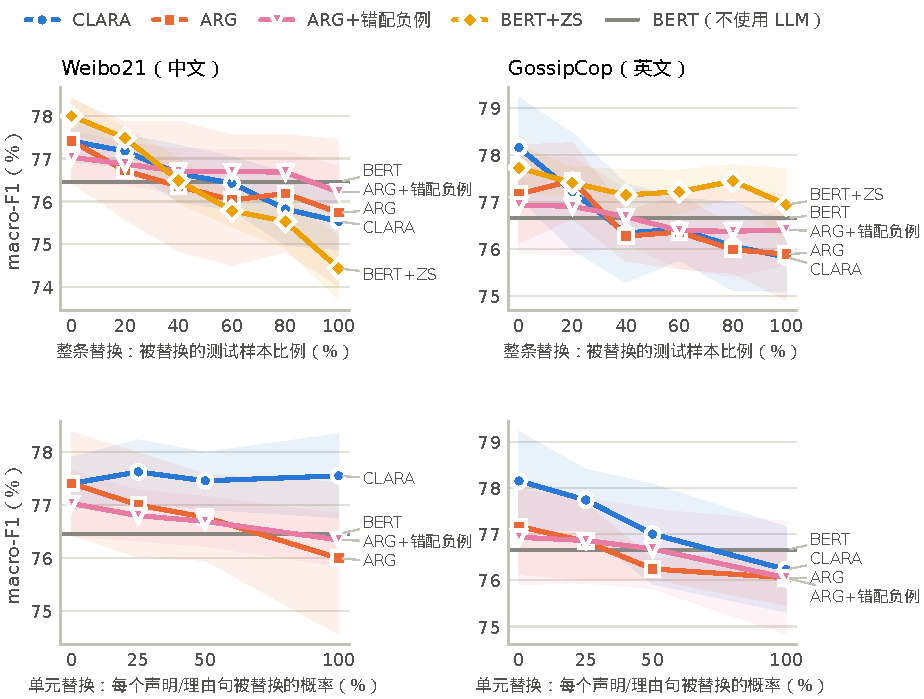
\includegraphics[width=\linewidth]{gen/figures/noise.pdf}
\caption{LLM 分析被替换时的 macro-F1}\label{fig:noise}
\note{上：整条替换；下：单元替换。阴影为种子间标准差，灰色横线为不使用 LLM 的 BERT。FactGuard 的下降幅度远大于其余方法，为保持纵轴的分辨率未画出；全部数值见表~\ref{tab:noise}。}
\end{figure}

\subsubsection{相关性门控能识别不属于该新闻的分析}
表~\ref{tab:gate} 显示，相关性门控 $r$ 几乎完美地区分了属于本新闻的分析单元与被替换进来的单元：整条替换时 AUC 为 \fthree{CN/gate/relevance/item/auc_r}（Weibo21）与 \fthree{EN/gate/relevance/item/auc_r}（GossipCop），单元替换时为 \fthree{CN/gate/relevance/unit/auc_r} 与 \fthree{EN/gate/relevance/unit/auc_r}。属于本新闻的单元平均 $r$ 在 0.93 以上，被替换的单元在 0.2 以下。判定门控 $g$ 则完全不具备这一能力（AUC 约 0.5）。

\begin{table}[htbp]
\centering\small
\caption{相关性门控对“分析单元是否属于该新闻”的区分能力}\label{tab:gate}
\fittable{gen/tables/gate.tex}
\note{测试集，多种子均值。}
\end{table}

\subsubsection{去掉相关性门控后模型在替换下崩溃}
消融实验（表~\ref{tab:ablation}）中“去掉相关性门控与错配负例”的变体，在全部分析被整条替换时，macro-F1 只有 \ptwo{CN/ablation/no_relevance/noise100/mean}（Weibo21）与 \ptwo{EN/ablation/no_relevance/noise100/mean}（GossipCop），远低于不使用 LLM 的 BERT。带相关性门控的完整模型在同样条件下为 \ptwo{CN/noise/clara/item/100/mean} 与 \ptwo{EN/noise/clara/item/100/mean}，比 BERT 低 \ptwo{CN/derived/clara_item100_gap} 与 \ptwo{EN/derived/clara_item100_gap} 个点。

\subsubsection{声明被逐条替换时，\method{} 可以丢弃声明而保留整体判断}
当分析中的声明被逐条替换时，\method{} 逐条关闭被替换声明的相关性门控，其余部分照常使用。在 Weibo21 上，即使全部声明都被替换，\method{} 的 macro-F1 仍为 \ptwo{CN/noise/clara/unit/100/mean}，与未替换时（\ptwo{CN/noise/clara/unit/0/mean}）持平。这一结果需要谨慎解读，因为两类方法在该条件下保留的信息不同：\method{} 的整体判断与零样本评分不由声明构成，因而没有被替换；ARG 的理由是一段自由文本，全部句子被替换后不再含有任何属于该新闻的 LLM 信息，这一条件对它几乎等同于整条替换（\ptwo{CN/noise/arg/unit/100/mean} 对 \ptwo{CN/noise/arg/item/100/mean}）。因此，此时 \method{} 比 ARG 高出的 \ptwo{CN/noise_sig/unit100/arg/diff_mean} 个点（$p_{\text{样本}}\peq{CN/noise_sig/unit100/arg/bootstrap/p}$，$p_{\text{种子}}\peq{CN/noise_sig/unit100/arg/welch_p}$；全精度复核中为 \ptwo{CN/fp32/clara_vs/arg_unit100/diff_mean} 个点，两种检验都成立，见附录~\ref{app:live}）说明的是结构上的一个性质：声明受到污染时，\method{} 可以只丢弃声明、继续使用整体判断；它并不说明在保留同等信息的条件下 \method{} 更稳健。当每个单元以一半的概率被替换时，两者相差 \ptwo{CN/noise_sig/unit50/arg/diff_mean} 个点，不显著。在 GossipCop 上，\method{} 从 \ptwo{EN/noise/clara/unit/0/mean} 降到 \ptwo{EN/noise/clara/unit/100/mean}，与 ARG（\ptwo{EN/noise/arg/unit/100/mean}）相当：如 \ref{sec:exp-gate} 节所示，该数据集上 \method{} 的判定更多依赖声明实例，丢弃声明的代价更大（\ref{sec:exp-ablation} 节的消融进一步显示，此时它低于从未使用声明的变体）。

\subsubsection{需要如实说明的两点}
第一，ARG 本身对替换就相当稳健：整条替换全部理由后，它在两个数据集上只下降 \ptwo{CN/derived/arg_item100_drop} 与 \ptwo{EN/derived/arg_item100_drop} 个点。它的融合权重并不能识别被替换的理由（被替换与未被替换样本上的平均权重几乎相同，区分两者的 AUC 为 \fthree{CN/gate/weights_under_noise/arg/auc} 与 \fthree{EN/gate/weights_under_noise/arg/auc}），稳健性来自新闻文本在其表示中占主导。给 ARG 加上同样的错配负例训练后，它在全部分析被整条替换时比 \method{} 高 \ptwo{CN/derived/argswap_minus_clara_item100}（Weibo21）与 \ptwo{EN/derived/argswap_minus_clara_item100}（GossipCop）个点，差异不显著。因此，“在分析不可用时保持稳健”并不是 \method{} 独有的性质：在两类方法都失去全部 LLM 信息的整条替换下，\method{} 与 ARG 没有差别。第二，FactGuard 对两种替换都非常敏感（整条替换全部分析后降到 \ptwo{CN/noise/factguard/item/100/mean} 与 \ptwo{EN/noise/factguard/item/100/mean}），因为它用 LLM 抽取的 topic-content 代替新闻原文参与交叉注意力。

\subsubsection{相关性门控识别的是话题层面的不匹配}
被替换进来的分析来自另一条新闻，与原文在话题上就不一致。为了检验相关性门控能否识别更细微的不匹配，我们把单句事实篡改集（\ref{sec:robust-sets} 节）中篡改后的文本与其\emph{原文}的 LLM 分析配对：此时分析与文本话题相同，只有对应被改句子的那条声明与文本在一处事实上不符。表~\ref{tab:cross} 显示相关性门控对此没有反应：对应被改句子的声明与其余声明的平均 $r$ 相同，用 $r$ 区分两者的 AUC 为 \fthree{CN/cross/cross/auc_r_unfaithful} 与 \fthree{EN/cross/cross/auc_r_unfaithful}。相关性门控能挡住的是“分析说的不是这条新闻”，挡不住“分析在某个事实上与这条新闻不符”。后者正是 LLM 幻觉更常见的形态，因此不能把相关性门控理解为对幻觉的一般性防护。

\begin{table}[htbp]
\centering\small
\caption{篡改后的文本搭配不同分析时的平均相关性门控 $r$}\label{tab:cross}
\fittable{gen/tables/cross.tex}
\note{分别搭配它自己的分析与原文的分析，按实例类别统计；3 个种子。}
\end{table}

\subsection{判定门控学到了什么}\label{sec:exp-gate}

判定门控 $g$ 的设计意图是估计“LLM 在该实例上是否站对了边”。表~\ref{tab:gate-cells} 按 LLM 的整体判断与新闻标签把测试样本分为四组，给出各组的平均 $g_0$。

\begin{table}[htbp]
\centering\small
\caption{判定门控在整体实例上的取值}\label{tab:gate-cells}
\fittable{gen/tables/gate_cells.tex}
\note{测试集，多种子均值。若门控跟随“LLM 是否正确”，则第一、四行应高，第二、三行应低。}
\end{table}

\subsubsection{判定门控跟随的是新闻标签，而不是 LLM 的正误}
在 Weibo21 上，$g_0$ 在两组假新闻上都高（约 0.81），在两组真新闻上都低（约 0.63--0.66），与 LLM 判断的方向无关：它预测“LLM 是否正确”的 AUC 为 \fthree{CN/gate/clara/overall/auc_gate/mean}，预测“新闻是否为假”的 AUC 却有 \fthree{CN/gate/clara/overall/auc_gate_for_label/mean}。在 GossipCop 上情形相反，$g_0$ 在真新闻上更高，对“LLM 是否正确”的 AUC 为 \fthree{EN/gate/clara/overall/auc_gate/mean}，但这同样可以由标签解释：该数据集上 LLM 多数时候判真，“LLM 正确”与“新闻为真”高度重合。也就是说，一个能看到新闻文本的门控学到的是“这条新闻像不像假新闻”，并据此调节 LLM 证据的权重。它起到的是让 LLM 证据的权重随文本先验变化的作用，而不是可靠性估计。

\subsubsection{这一现象并非 \method{} 独有}
ARG 的理由可用性预测器对“该理由对应的 LLM 判断是否正确”的 AUC 看起来不低（表~\ref{tab:useful}），但决定融合权重的打分模块对同一目标的 AUC 只有 0.50--0.55（加入错配负例训练后为 0.45--0.67）。可用性预测器同时读取新闻与理由：新闻文本提示标签，理由文本提示 LLM 的判断，两者一比较即可得到监督目标。表中“自身预测”一列用 ARG 最终的预测概率与 LLM 判断是否一致来预测同一目标，不需要任何专门的模块，得到的 AUC 与可用性预测器相当或更高。可见可用性预测器并没有提供分类器自身判断之外的信息。

\begin{table}[htbp]
\centering\small
\caption{对“该理由对应的 LLM 判断是否正确”的 AUC}\label{tab:useful}
\fittable{gen/tables/useful.tex}
\note{测试集，多种子均值。三列分别为 ARG 的可用性预测器、融合权重，以及“ARG 自身的最终预测与 LLM 判断是否一致”。}
\end{table}

\subsubsection{LLM 自身的置信度也不提供这一信息}
LLM 评分偏离 0.5 的程度对其判断是否正确的 AUC 只有 \fthree{CN/gate/clara/overall/auc_llm_conf/mean} 与 \fthree{EN/gate/clara/overall/auc_llm_conf/mean}。真正有信息量的是“文本分支是否同意 LLM”（AUC \fthree{CN/gate/clara/overall/auc_text_agreement/mean} 与 \fthree{EN/gate/clara/overall/auc_text_agreement/mean}），而这一信息在加性融合中已经被隐式使用。综合来看，在闭卷条件下我们没有找到能够估计“LLM 的判断是否可靠”且不退化为预测标签的信号；本文最初设想的“声明级可靠性门控”在这一含义上没有成立，成立的是相关性门控所回答的那个更窄的问题。

\subsubsection{实例概率的分布}
两个数据集上承担判定的实例不同。在 Weibo21 的假新闻中，至少有一条声明 $p_k>0.5$ 的占 \pone{CN/gate/clara/flag/fake_any_claim/mean}\%，只有整体实例 $p_0>0.5$ 的占 \pone{CN/gate/clara/flag/fake_overall_only/mean}\%，可见这里新闻级的判定主要由整体实例承担。在 GossipCop 的假新闻中，至少有一条声明 $p_k>0.5$ 的占 \pone{EN/gate/clara/flag/fake_any_claim/mean}\%，而只由整体实例触发的不到 1\%：该数据集上 LLM 的整体判断区分度很低（零样本判断的 AUC 仅 \pone{EN/style_llm/zero-shot P(fake)/auc_orig}\%），裁决器转而依靠声明实例。

\subsection{风格改写}\label{sec:exp-style}

\begin{table}[htbp]
\centering\small
\caption{风格改写前后的 macro-F1（\%）}\label{tab:style}
\fittable{gen/tables/style.tex}
\note{只统计成功改写的样本，“原文”为同一批样本改写前的结果。分隔线以下两行是只读取 LLM 输出文本、不读新闻原文的 BERT。}
\end{table}

\subsubsection{所有闭卷检测器都主要依赖文风}
把假新闻改写为通稿文风、真新闻改写为营销号文风后，Weibo21 上所有 SLM 类方法的 macro-F1 从 76--78 降到 50--53，接近随机；GossipCop 上从 77--78 降到 65--69（表~\ref{tab:style}）。读取 LLM 理由并不能使检测器摆脱对文风的依赖。在 Weibo21 上，改写后各 SLM 类方法与 BERT 的差异都不显著。在 GossipCop 上，FactGuard 与 \method{} 改写后分别比 BERT 高 \ptwo{EN/style/_vs_bert/factguard/diff_mean} 与 \ptwo{EN/style/_vs_bert/clara/diff_mean} 个点，差异显著；这两种方法都使用了 LLM 对新闻内容的重新表述（topic-content 或声明），其文风与原文不同，ARG 则没有这一差别（\ptwo{EN/style/_vs_bert/arg/diff_mean} 个点）。直接微调的 LoRA-LLM 下降最少（Weibo21 上 \ptwo{CN/derived/lora_style_drop} 个点，GossipCop 上 \ptwo{EN/derived/lora_style_drop} 个点），改写后在两个数据集上都显著高于 BERT，但在 Weibo21 上也只剩 \ptwo{CN/style/lora/style/mean}。

\subsubsection{只读 LLM 复述的分类器：更稳健，但暴露了分布内精度的来源}
表~\ref{tab:style} 分隔线以下的两行是不读新闻原文、只读 LLM 输出的 BERT：一行读 FactGuard 式的 topic-content 摘要，一行读 \method{} 抽取的声明。在 GossipCop 上，只读摘要的 BERT 在原始测试集上为 \ptwo{EN/main/bert_tc/macf1}，不低于读原文的 BERT（\ptwo{EN/main/bert/macf1}），风格改写后仍有 \ptwo{EN/style/bert_tc/style/mean}，比读原文的 BERT 高 \ptwo{EN/style/_vs_bert/bert_tc/diff_mean} 个点；只读声明的 BERT 改写后为 \ptwo{EN/style/bert_claims/style/mean}。在 Weibo21 上，只读摘要的 BERT 改写后为 \ptwo{CN/style/bert_tc/style/mean}，同样显著高于读原文的 BERT（\ptwo{CN/style/bert/style/mean}），但它在原始测试集上只有 \ptwo{CN/main/bert_tc/macf1}，比读原文低 \ptwo{CN/derived/bert_minus_bert_tc} 个点。这两个数值与 FactGuard 论文中“仅用 topic-content”的消融结果（69.0 与 76.9）\citep{he2026factguard}一致。它们说明两点：第一，让 LLM 先用中性的措辞复述新闻，确实能削弱检测器对文风的依赖；第二，在 Weibo21 上，去掉文风的代价约为 6 个点，分布内精度中有相当一部分来自文风。声明并不总是风格中性的：在以短帖为主的 Weibo21 上，LLM 抽取的声明基本沿用原文措辞，只读声明的 BERT 改写后只有 \ptwo{CN/style/bert_claims/style/mean}，低于随机。

\subsubsection{LLM 自身的判断同样依赖文风}
表~\ref{tab:style-llm} 不涉及任何训练，只比较 Qwen2.5-7B 对同一批样本改写前后的评分。零样本判断的 AUC 在 Weibo21 上从 \pone{CN/style_llm/zero-shot P(fake)/auc_orig} 降到 \pone{CN/style_llm/zero-shot P(fake)/auc_style}，在 GossipCop 上从 \pone{EN/style_llm/zero-shot P(fake)/auc_orig} 降到 \pone{EN/style_llm/zero-shot P(fake)/auc_style}。声明级怀疑度在改写后对真假新闻几乎没有区分度。这说明 LLM 在闭卷条件下给出的“常识分析”“声明核查”，其判别力主要来自文本的表面特征，而不是对事实的掌握。把 LLM 的分析拆得更细并不能改变这一点：声明是从改写后的文本中抽取的，其措辞与评分仍然随文风变化。

\begin{table}[htbp]
\centering\small
\caption{Qwen2.5-7B 的评分在风格改写前后对真假新闻的区分能力}\label{tab:style-llm}
\fittable{gen/tables/style_llm.tex}
\note{不涉及训练。均值差为假新闻与真新闻平均评分之差。}
\end{table}

\subsection{单句事实篡改：敏感性与定位}\label{sec:exp-loc}

\begin{table}[htbp]
\centering\small
\caption{各方法对单句事实篡改的敏感性（\%）}\label{tab:tamper}
\fittable{gen/tables/tamper.tex}
\note{“判假”为被判为假的比例；成对正确率为篡改后样本的预测概率高于其原文的比例，50\% 相当于随机。}
\end{table}

\subsubsection{SLM 类方法对局部事实改动几乎没有反应}
表~\ref{tab:tamper} 显示，把真新闻中的一句话改成与原文事实不符的陈述后，各 SLM 类方法判其为假的比例几乎不变（例如 \method{} 在 Weibo21 上从 \pone{CN/localisation/_sensitivity/clara/flag_rate_original}\% 变为 \pone{CN/localisation/_sensitivity/clara/flag_rate_tampered}\%）；篡改后的预测概率高于原文的比例只有 53\%--55\%，略高于随机。BERT+ZS 稍高（\pone{CN/localisation/_sensitivity/bert_zs/pairwise_acc}\% 与 \pone{EN/localisation/_sensitivity/bert_zs/pairwise_acc}\%），因为 LLM 的零样本评分对部分改动有反应。直接微调的 LoRA-LLM 最敏感，成对正确率为 \pone{CN/localisation/_sensitivity/lora/pairwise_acc}\% 与 \pone{EN/localisation/_sensitivity/lora/pairwise_acc}\%，但它判假的比例同样变化很小（Weibo21 上从 \pone{CN/localisation/_sensitivity/lora/flag_rate_original}\% 到 \pone{CN/localisation/_sensitivity/lora/flag_rate_tampered}\%）：预测概率朝正确的方向移动了，幅度却远不足以改变判定。这与风格改写的结果一致：这些检测器学到的主要不是“内容是否属实”。需要强调，篡改后的句子只是与原文不符，未必在现实中为假，这项测试衡量的是模型对事实内容变化的敏感程度。

\begin{table}[htbp]
\centering\small
\caption{被篡改句子的定位结果（\%）}\label{tab:loc}
\fittable{gen/tables/loc.tex}
\note{“单位”为方法给出分数的粒度；声明级分数通过声明所在的句子编号映射到句子。分隔线以下为 \method{} 与 \student{} 的消融变体。}
\end{table}

\subsubsection{定位结果只略高于随机}
在定位任务上（表~\ref{tab:loc}），\method{} 的 Hit@1 在 Weibo21 上为 \pone{CN/localisation/CLARA/hit@1}\%，随机猜测为 \pone{CN/localisation/CLARA/chance}\%；在 GossipCop 上为 \pone{EN/localisation/CLARA/hit@1}\%，随机为 \pone{EN/localisation/CLARA/chance}\%。训练后的裁决器并没有比直接使用 LLM 的怀疑度评分更好（\pone{CN/localisation/LLM suspicion scores/hit@1}\% 与 \pone{EN/localisation/LLM suspicion scores/hit@1}\%），各消融变体也都在同一水平。表中最好的是对 LoRA-LLM 做遮挡归因（Weibo21 上 \pone{CN/localisation/LoRA-LLM + occlusion/hit@1}\%），它不需要任何声明级结构。\method{} 的定位受两方面限制：LLM 抽取的声明只覆盖了 \pone{CN/localisation/_claim_coverage}\%（Weibo21）与 \pone{EN/localisation/_claim_coverage}\%（GossipCop）的被篡改句子；即使覆盖到，LLM 对这条声明的怀疑度也往往不比其他声明高。“只用新闻级标签即可获得声明级定位”这一预期在闭卷条件下没有实现。

\subsection{消融实验}\label{sec:exp-ablation}

\begin{table}[htbp]
\centering\footnotesize
\setlength{\tabcolsep}{3.4pt}
\caption{\method{} 的消融实验（macro-F1，\%）}\label{tab:ablation}
\fittable{gen/tables/ablation.tex}
\note{“整条替换”与“单元替换”分别为全部测试样本的分析被整条替换、全部声明被逐条替换时的结果。Weibo21 为 5 个种子，GossipCop 为 3 个种子。$^{*}$ 表示在同一评测条件下与完整模型的差异显著（两种检验均 $p<0.05$，未做多重比较校正）。}
\end{table}

表~\ref{tab:ablation} 逐一去掉或替换 \method{} 的组件。Weibo21 为 5 个种子；GossipCop 为 \cnt{EN/ablation/_seeds_count} 个种子，表中“完整”一行取同样的种子（\ptwo{EN/ablation/full/test/mean}），因此与表~\ref{tab:main} 中 5 个种子的数值不同。

\subsubsection{两个数据集上一致的结论：论证文本、声明分解与判定门控对精度没有可测的贡献}
去掉全部论证文本、只保留评分，macro-F1 在 Weibo21 上为 \ptwo{CN/ablation/no_args/test/mean}（完整模型 \ptwo{CN/ablation/full/test/mean}），在 GossipCop 上为 \ptwo{EN/ablation/no_args/test/mean}（完整模型 \ptwo{EN/ablation/full/test/mean}），差异都不显著。只保留整体实例而去掉全部声明（\ptwo{CN/ablation/no_claims/test/mean} 与 \ptwo{EN/ablation/no_claims/test/mean}）、去掉判定门控（\ptwo{CN/ablation/no_gate/test/mean} 与 \ptwo{EN/ablation/no_gate/test/mean}）、整条新闻共用一个判定门控、把 noisy-OR 换成注意力聚合、允许实例证据读取整条新闻，在原始测试集上与完整模型的差异同样都不显著。本文方法的核心设想是让小模型阅读并裁决声明级的正反论证；就分布内精度而言，这一设想中的每个部件都可以去掉而不产生可测的损失。

\subsubsection{LLM 评分的作用因数据集而异}
在 Weibo21 上，去掉评分、只保留论证文本，macro-F1 降到 \ptwo{CN/ablation/no_v/test/mean}，显著低于完整模型，也低于不使用 LLM 的 BERT（\ptwo{CN/main/bert/macf1}）；把论证前的整体评分从零样本判断换成提示内的第一印象（即严格的单次调用），降到 \ptwo{CN/ablation/fi_score/test/mean}，同样显著。也就是说，在这个数据集上 \method{} 相对 BERT 的提升几乎全部来自 LLM 的数值评分，尤其是单独一次调用得到的零样本评分，这与 BERT+ZS 的结果（\ref{sec:main-results} 节）相互印证。在 GossipCop 上情形不同：去掉评分后为 \ptwo{EN/ablation/no_v/test/mean}，换成第一印象后为 \ptwo{EN/ablation/fi_score/test/mean}，都不显著。该数据集上 LLM 评分的区分度本来就低（零样本判断的 AUC 为 \pone{EN/style_llm/zero-shot P(fake)/auc_orig}\%）。除整体文本分支外，GossipCop 上没有任何单个组件的去除造成显著下降，\method{} 相对 BERT 的差距（本身不显著）无法归因到某个具体组件。

\subsubsection{相关性门控与整体文本分支决定了稳健性}
去掉相关性门控与错配负例不显著影响原始测试集上的精度（\ptwo{CN/ablation/no_relevance/test/mean} 与 \ptwo{EN/ablation/no_relevance/test/mean}），但全部分析被整条替换时，macro-F1 降到 \ptwo{CN/ablation/no_relevance/noise100/mean} 与 \ptwo{EN/ablation/no_relevance/noise100/mean}，比完整模型低 \ptwo{CN/ablation/no_relevance/vs_full_noise100/diff_mean} 与 \ptwo{EN/ablation/no_relevance/vs_full_noise100/diff_mean} 个点，比 BERT 低 \ptwo{CN/derived/no_relevance_gap} 与 \ptwo{EN/derived/no_relevance_gap} 个点。整体文本分支是唯一在两个数据集的原始测试集上都显著的组件（去掉后下降 \ptwo{CN/ablation/no_global/vs_full/diff_mean} 与 \ptwo{EN/ablation/no_global/vs_full/diff_mean} 个点）；没有它，分析被整条替换时模型在 GossipCop 上降到 \ptwo{EN/ablation/no_global/noise100/mean}，相当于恒定预测。

\subsubsection{丢弃被替换的声明并不总是没有代价}
\ref{sec:exp-noise} 节指出，声明被逐条替换时 \method{} 可以丢弃声明、依靠整体实例。Weibo21 上的消融印证了这一机制：去掉整体实例的变体在全部声明被替换时降到 \ptwo{CN/ablation/no_overall/unit100/mean}，显著低于完整模型（\ptwo{CN/ablation/full/unit100/mean}）。但在 GossipCop 上，完整模型在同一条件下为 \ptwo{EN/ablation/full/unit100/mean}，显著低于从一开始就不使用声明的变体（\ptwo{EN/ablation/no_claims/unit100/mean}，该变体不受声明替换影响）。相关性门控识别出了被替换的声明，但裁决器在该数据集上平时依赖声明实例（\ref{sec:exp-gate} 节），退回之后的表现不如从未使用声明的模型。

\subsection{学生模型}\label{sec:exp-distill}

\begin{table}[htbp]
\centering\small
\caption{推理时不调用 LLM 的学生模型（macro-F1，\%）}\label{tab:distill}
\fittable{gen/tables/distill.tex}
\note{3 个种子。“其教师”为同一次运行中训练的教师模型的结果；$^{*}$ 表示与同样种子的 BERT 相比差异显著。}
\end{table}

\subsubsection{蒸馏得到的学生都没有显著超过 BERT}
表~\ref{tab:distill} 给出三种方法的学生模型。在 Weibo21 上，ARG-D（\ptwo{CN/distill/arg_d/test/mean}）与同样种子的 BERT（\ptwo{CN/distill/bert/test/mean}）持平，FactGuard-D（\ptwo{CN/distill/factguard_d/test/mean}）与 \student{}（\ptwo{CN/distill/clara_d/test/mean}）略低，差异都不显著。在 GossipCop 上 \student{} 为 \ptwo{EN/distill/clara_d/test/mean}，比 BERT 高 \ptwo{EN/distill/clara_d/vs_bert/diff_mean} 个点，但差异不显著（$p_{\text{样本}}\peq{EN/distill/clara_d/vs_bert/bootstrap/p}$，$p_{\text{种子}}\peq{EN/distill/clara_d/vs_bert/welch_p}$）；ARG-D 与 BERT 持平，FactGuard-D 更低。各教师模型本身相对同种子 BERT 的优势只有 0.3--1.6 个点且大多不显著，学生再损失一部分之后，“把 LLM 的知识蒸馏进小模型”在本文的设置下没有留下可测的收益。原论文报告 ARG-D 比 BERT 高约 1.3--1.8 个点\citep{hu2024bad}，在本文的多种子复现中没有重现。

\subsubsection{声明到句子的对齐蒸馏没有带来定位能力}
\student{} 的设计目标之一是保留句级定位。表~\ref{tab:loc} 显示这一目标没有实现：它在 Weibo21 上的 Hit@1 为 \pone{CN/localisation/CLARA-D/hit@1}\%，与随机猜测（\pone{CN/localisation/CLARA-D/chance}\%）相同；在 GossipCop 上为 \pone{EN/localisation/CLARA-D/hit@1}\%（随机 \pone{EN/localisation/CLARA-D/chance}\%）。去掉实例级蒸馏、甚至完全不用教师的句子级 MIL 变体，定位结果都在同一水平。教师的声明级概率本身几乎不含位置信息（\ref{sec:exp-loc} 节），对齐到句子之后自然无从蒸馏。

\subsection{未见领域}\label{sec:exp-lodo}

\begin{table}[htbp]
\centering\small
\caption{Weibo21 留一领域实验的 macro-F1（\%）}\label{tab:lodo}
\fittable{gen/tables/lodo.tex}
\note{3 个种子；训练与验证数据不含被留出的领域。每行最优者加粗，$^{*}$ 表示各领域平均值显著高于 BERT。}
\end{table}

表~\ref{tab:lodo} 给出六个领域的留一领域结果。各领域的测试集只有一百到四百条，单个领域上的数值波动很大，下面只讨论各领域的平均值；它的检验采用按领域分层的 bootstrap 与对种子的 Welch 检验。

\subsubsection{在未见领域上有帮助的仍然是 LLM 的零样本评分}
BERT+ZS 的平均 macro-F1 为 \ptwo{CN/lodo/_macro_avg/bert_zs}，比 BERT 高 \ptwo{CN/derived/lodo_bert_zs_minus_bert} 个点，差异显著（$p_{\text{样本}}\peq{CN/lodo/_vs_bert/bert_zs/bootstrap/p}$，$p_{\text{种子}}\peq{CN/lodo/_vs_bert/bert_zs/welch_p}$），在六个领域中的四个上最高。LLM 的判断不依赖训练数据的领域分布，把它作为一个加性的先验，领域变化时仍然有效。

\subsubsection{\method{} 与 ARG 在未见领域上没有超过 BERT}
ARG 与 \method{} 的平均值为 \ptwo{CN/lodo/_macro_avg/arg} 与 \ptwo{CN/lodo/_macro_avg/clara}，与 BERT（\ptwo{CN/lodo/_macro_avg/bert}）没有差别。\method{} 显著低于 BERT+ZS（相差 \ptwo{CN/derived/lodo_clara_minus_bert_zs} 个点，$p_{\text{样本}}\peq{CN/lodo/_vs_bert_zs/clara/bootstrap/p}$，$p_{\text{种子}}\peq{CN/lodo/_vs_bert_zs/clara/welch_p}$），尽管它同样读入了零样本评分。一个可能的原因是，\method{} 对该评分的使用要经过在训练领域上拟合的门控与证据模块（\ref{sec:exp-gate} 节显示判定门控跟随的是文本的标签倾向），这些模块本身带有领域依赖；而 BERT+ZS 只用一个标量权重。这是更复杂的协同结构相对简单融合的一个明确的劣势。

\subsection{拒答}\label{sec:exp-selective}

\begin{table}[htbp]
\centering\small
\caption{选择性预测的结果}\label{tab:selective}
\fittable{gen/tables/selective.tex}
\note{多种子均值。AURC 越低越好；其余各列为只保留置信度最高的一部分样本时的准确率（\%），覆盖率 100\% 即不拒答。“选择器”为在验证集上拟合的逻辑回归。}
\end{table}

\begin{figure}[htbp]
\centering
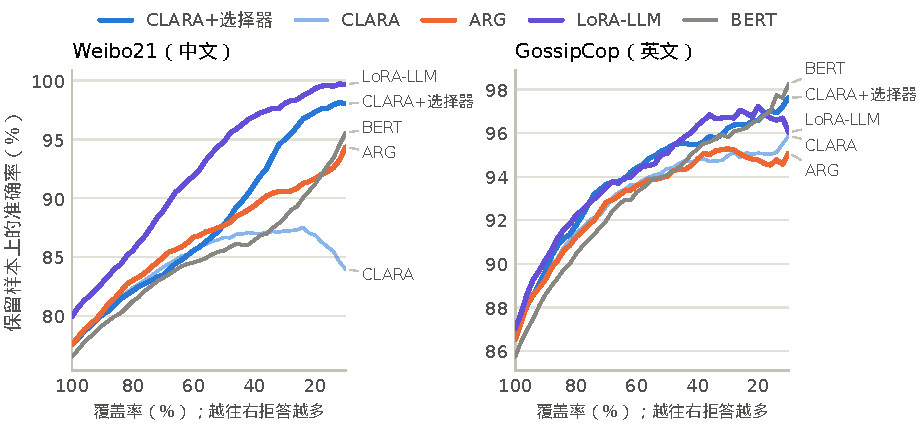
\includegraphics[width=\linewidth]{gen/figures/selective.pdf}
\caption{保留样本上的准确率随覆盖率的变化}\label{fig:selective}
\note{多种子均值。浅色线为 \method{} 直接用 $|\hat y-0.5|$ 作为置信度的结果；数值见表~\ref{tab:selective}。}
\end{figure}

\subsubsection{直接使用 LLM 评分会损害置信度排序}
表~\ref{tab:selective} 中，以 $|\hat y-0.5|$ 为置信度时，Weibo21 上 \method{} 的 AURC（\ptwo{CN/selective/clara/maxprob/aurc}）比 BERT（\ptwo{CN/selective/bert/maxprob/aurc}）更差，BERT+ZS 与 FactGuard 也是如此。问题出在最有把握的那部分预测：只保留置信度最高的 10\% 样本时，BERT 的准确率为 \pone{CN/selective/bert/maxprob/acc@10}\%，\method{} 只有 \pone{CN/selective/clara/maxprob/acc@10}\%，BERT+ZS 为 \pone{CN/selective/bert_zs/maxprob/acc@10}\%。原因在于 LLM 的零样本评分高度两极化而且过于自信：Weibo21 测试集中有 \pone{CN/zs_calibration/hi_share}\% 的样本 $p_{\mathrm{zs}}>0.95$，其中实际为假的只有 \pone{CN/zs_calibration/hi_fake_rate}\%。把它的 logit 加到输出上，这批样本就被整体推到置信度的最高端：\method{} 置信度最高的 10\% 预测中有 \pone{CN/selective/clara/maxprob/top10_fake_share}\% 判假（BERT 为 \pone{CN/selective/bert/maxprob/top10_fake_share}\%），这一侧的准确率只有 \pone{CN/selective/clara/maxprob/top10_acc_fake_side}\%，判真的一侧则为 \pone{CN/selective/clara/maxprob/top10_acc_real_side}\%。\method{} 与 BERT+ZS 都没有对 LLM 的评分做校准，这是两者共同的缺陷。GossipCop 上 LLM 很少给出接近 1 的评分（$p_{\mathrm{zs}}>0.95$ 的样本占 \pone{EN/zs_calibration/hi_share}\%），这一现象不明显。

\subsubsection{选择器可以修复这一问题，但不构成优势}
用裁决器的内部信号在验证集上拟合选择器后，\method{} 在 Weibo21 上的 AURC 降到 \ptwo{CN/selective/clara/selector/aurc}，置信度最高的 10\% 样本准确率回到 \pone{CN/selective/clara/selector/acc@10}\%。这一 AURC 在 SLM 类方法中数值最低：对随机种子的 Welch 检验显示它低于 BERT 与 BERT+ZS（$p\peq{CN/selective/_selector_vs/bert/maxprob/welch_p}$ 与 $\fthree{CN/selective/_selector_vs/bert_zs/maxprob/welch_p}$），但与同样拟合了选择器的 ARG（\ptwo{CN/selective/arg/selector/aurc}）没有可分辨的差别（$p\peq{CN/selective/_selector_vs/arg/selector/welch_p}$），并且远不及 LoRA-LLM（\ptwo{CN/selective/lora/maxprob/aurc}）。AURC 没有做对测试样本的 bootstrap，这些 $p$ 值只供参考。覆盖率为 50\% 时，\method{} 加选择器的准确率为 \pone{CN/selective/clara/selector/acc@50}\%，ARG 加选择器为 \pone{CN/selective/arg/selector/acc@50}\%。GossipCop 上各方法的 AURC 都在 5--7 之间，BERT+ZS 最低（\ptwo{EN/selective/bert_zs/maxprob/aurc}），\method{} 加选择器为 \ptwo{EN/selective/clara/selector/aurc}。总体上，\method{} 的内部信号可以用来纠正它自身的置信度排序，但没有带来超出其他方法的拒答能力；原设想中“两分支分歧与门控提供不可判信号”没有得到支持。

\subsection{更换分析用的 LLM}\label{sec:exp-llm2}

\begin{table}[htbp]
\centering\footnotesize
\setlength{\tabcolsep}{3.6pt}
\caption{更换分析用 LLM 后的 macro-F1（\%）}\label{tab:llm2}
\fittable{gen/tables/llm2.tex}
\note{把 Qwen2.5-7B 换成 Qwen3-8B，3 个种子（Qwen2.5 一列取相同的种子）；各方法沿用在 Qwen2.5 上选出的学习率。“整条替换”为全部测试样本的 LLM 输出被替换。}
\end{table}

为了检验结论是否依赖于某一个 LLM，我们用 Qwen3-8B（关闭思考模式）重新生成全部 LLM 输出，并重新训练依赖 LLM 输出的四种方法（表~\ref{tab:llm2}）。

\subsubsection{分布内的结论不变}
换用 Qwen3-8B 后，四种方法在两个数据集上的变化都在 1.5 个点以内，彼此之间仍然相差不到 2 个点。在两个 LLM 与两个数据集构成的四种组合中，\method{} 在三种上数值最高（Weibo21 上使用 Qwen2.5 时 BERT+ZS 最高），但对第二名的领先都不到 1 个点，在 3 个种子下不足以说明问题。

\subsubsection{相关性门控是软门控，残余的泄漏随运行而变}
换用 Qwen3-8B 后，相关性门控区分两类分析单元的 AUC 仍在 0.99 左右，但被替换单元上的平均 $r$ 在 Weibo21 上从 \ftwo{CN/llm2/relevance_first/item/r_foreign} 升到 \ftwo{CN/llm2/relevance_second/item/r_foreign}：门控把它们排在了后面，却没有把它们压到接近 0。由于 $r$ 是连续的乘性系数，这些单元的证据仍有一部分进入判定，\method{} 在全部分析被整条替换时降到 \ptwo{CN/llm2/clara/second_noise100/mean}，低于同条件下的 ARG（\ptwo{CN/llm2/arg/second_noise100/mean}）与不使用 LLM 的 BERT。在 GossipCop 上情形相反，\method{} 为 \ptwo{EN/llm2/clara/second_noise100/mean}，ARG 降到 \ptwo{EN/llm2/arg/second_noise100/mean}。因此，\ref{sec:exp-noise} 节中“整条替换下 \method{} 与 ARG 相当”的结论，更准确的表述是两者互有高低、没有系统性的差别；\method{} 的退回并不精确，其程度取决于门控被压低的幅度。推理时对 $r$ 取硬阈值可能缓解这一问题，本文没有验证。

\subsection{开销}\label{sec:exp-cost}

\begin{table}[htbp]
\centering\small
\caption{每条新闻的 LLM 开销}\label{tab:cost}
\fittable{gen/tables/cost.tex}
\note{平均输入与输出 token 数，以及单张 RTX 3090 上用 vLLM 批量生成时每千条新闻的耗时（秒）。$^\ddagger$ LoRA-LLM 的耗时用 Transformers 逐批前向测得，与 vLLM 不是同一推理实现，仅供量级参考。}
\end{table}

\begin{table}[htbp]
\centering\small
\caption{可训练参数量与单次训练耗时}\label{tab:train-cost}
\fittable{gen/tables/train_cost.tex}
\note{单张 RTX 3090；SLM 类方法使用冻结层缓存与混合精度，不含一次性的缓存构建。}
\end{table}

\subsubsection{\method{} 的 LLM 开销高于 ARG 与 FactGuard}
表~\ref{tab:cost} 显示，\method{} 的结构化调用要为每条声明输出两条论证，是各方法中最贵的：其输出 token 数在 Weibo21 上是 ARG 两条理由之和的 \ftwo{CN/cost/clara_over_arg/completion} 倍，在新闻更长、声明更多的 GossipCop 上是 \ftwo{EN/cost/clara_over_arg/completion} 倍；生成耗时分别是 \ftwo{CN/cost/clara_over_arg/seconds_per_1000} 倍与 \ftwo{EN/cost/clara_over_arg/seconds_per_1000} 倍。把辩论压缩到一次结构化调用，相对于每条新闻需要多次调用的辩论方法节省了调用次数，但相对于只需两段短理由的 ARG 与 FactGuard 并不便宜。BERT+ZS 只需要一次输出单个 token 的调用，是使用 LLM 的方法中最便宜的，而它的精度并不低（表~\ref{tab:main}）。

\subsubsection{训练与推理}
LoRA-LLM 推理时只做一次前向，开销与零样本判断同一量级，但需要对 7B 模型做一次约 \cnt{CN/lora_cost/train_seconds} 秒（Weibo21）的微调，并在部署时常驻一个 7B 模型。SLM 类方法在缓存冻结层之后单次训练不到 3 分钟（表~\ref{tab:train-cost}）；其中 ARG、FactGuard 与 \method{} 推理前都需要先完成表~\ref{tab:cost} 中的 LLM 生成。

\section{讨论}\label{sec:discussion}

\subsubsection{LLM 的理由文本为什么没有帮助}
消融实验中最直接的一条结果是：把 LLM 写的论证文本全部去掉、只留下它给出的评分，\method{} 在两个数据集上的精度都没有显著变化。BERT+ZS 与 ARG、FactGuard 的比较给出了同样的信息。一种解释是，在闭卷条件下 LLM 的分析文本本身不携带新闻原文之外的新信息：它是 LLM 对同一段文字的复述与评价，其中对判别有用的部分可以被压缩成一个倾向性分数，而小模型已经直接读到了新闻原文。分析文本只有在引入原文之外的内容（例如检索到的证据、LLM 确实掌握的背景事实）时才可能提供增量；\ref{sec:exp-style} 节的结果表明，至少对 7B 模型而言，后者很有限。

\subsubsection{为什么判定门控学不到“LLM 是否可靠”}
“LLM 在某个实例上是否站对了边”由两个量决定：LLM 表达的判断与该实例的真实状态。前者写在 LLM 的输出里，后者在闭卷条件下只能由新闻文本去推测。因此，一个读取新闻文本与 LLM 输出的门控，要预测这一目标，最直接的办法就是先从文本预测标签，再与 LLM 的判断比较。表~\ref{tab:gate-cells} 与表~\ref{tab:useful} 显示 \method{} 的判定门控与 ARG 的可用性预测器都落在这一解上。要得到不依赖标签预测的可靠性估计，需要第三个信息来源，例如外部证据，或 LLM 在同一问题上多次采样的一致性；后者是否有效留待后续工作检验。多示例学习的不对称性确实为真新闻中的声明提供了精确的监督，但这一监督同样可以由“这是一条真新闻”推出，并没有迫使模型去判断单条声明。

\subsubsection{多示例假设在多大程度上成立}
式~\eqref{eq:mil} 假设假新闻中存在可以单独指认的问题声明。\ref{sec:exp-gate} 节的统计显示，在 Weibo21 上多数假新闻是由整体实例而不是某条声明触发的。这与数据的性质有关：社交媒体上的不实消息常常整体是编造的，其中每条声明单独看都“像是可能发生的”，仅凭文本无法指出哪一条有问题。反过来，真新闻如实转述不实说法的情形会违反假设的另一半；我们在提示词中要求保留归属以减少这种情况，但没有通过人工标注去度量假设被违反的比例，这是本文的一个局限。

\subsubsection{关于任务本身}
风格改写与事实篡改两项测试指向同一个结论：在这两个常用数据集上，闭卷检测器学到的主要是真假新闻在写法上的差异。这与 Wu 等\citep{wu2024sheepdog}对 SLM 的观察一致，本文进一步表明它同样适用于 LLM 的闭卷判断，以及建立在这些判断之上的协同方法。把 LLM 的分析拆得更细、让它写出正反论证，改变的是分析的形式，而没有改变分析所依据的信息。对于“内容是否属实”这一问题，闭卷的 7B 模型既不掌握所需的事实，也没有表现出能从文本内部一致性中发现问题的能力。这提示：在不引入外部证据的前提下继续改进 LLM 与 SLM 的协同结构，在这类基准上能得到的主要是对文风线索更充分的利用；而声称具备“事实分析”能力的闭卷方法，应当接受风格受控的测试。

\subsubsection{对实践的建议}
如果目标只是分布内精度：在算力允许时直接微调 LLM；否则在 SLM 的输出上融合一个 LLM 零样本评分，成本最低且不逊于更复杂的结构。如果系统中确实要使用 LLM 生成的分析文本，本文的结果支持为它配一个相关性检查：它几乎不损失精度，却能避免在分析与新闻不符时性能大幅下降。无论采用哪种方案，方法间 1 个点以内的差异都需要多个随机种子与显著性检验才能判断。

\subsubsection{局限}
（1）分析用的 LLM 以 Qwen2.5-7B 为主，更强的模型可能掌握更多事实，结论未必外推到闭源大模型。（2）只使用了两个数据集，且都来自同一来源的时间划分。（3）风格改写与事实篡改由另一个 LLM 自动生成，事实是否保持只用数字串的保留比例做了粗略检查，没有人工核验；篡改后的句子与原文不符，但未必在现实中为假。生成这两个测试集的 Qwen3-8B 同时是 \ref{sec:exp-llm2} 节中的第二个分析模型，因此更换 LLM 的实验没有在这两个测试集上评测。（4）\method{} 的第一个版本曾在测试集上评估过一次，相关性门控是在看到那次结果后加入的（\ref{sec:protocol} 节）；虽然此后的选择只依据验证集，这仍然弱化了测试集的独立性。（5）主实验为节省算力使用了混合精度。全精度复核（附录~\ref{app:live}）没有改变定性结论，但显示 ARG 与 FactGuard 的数值对精度敏感，使用 GPT-3.5 理由的 ARG 在混合精度下比官方代码低 \ptwo{CN/official_arg/gap_cached} 个点；正文中 1 个点左右的差异不应被解读为方法之间的排序。（6）声明的质量、论证的质量以及定位结果都没有做人工评估。（7）\method{} 的超参数没有搜索，可能不是最优。

\section{本章小结}\label{sec:ch3-summary}

本章研究了闭卷条件下如何利用 LLM 的分析来检测虚假新闻，提出了声明级论证裁决方法 \method{}，并在统一 LLM、超参数搜索与随机种子的条件下，把它与 ARG、FactGuard、直接微调的 LLM 以及一个简单的评分融合基线做了比较。结论可以概括为三点。

第一，就方法而言，\method{} 在分布内与已有的协同方法持平，在未见领域上不如只融合一个 LLM 评分的简单基线；消融显示，论证文本、声明分解与判定门控对精度都没有可测的贡献。它的相关性门控是有效的，能可靠地识别与新闻对不上的分析单元，但回答的只是“分析是否属于这条新闻”，而不是“分析是否正确”。

第二，就这一类方法而言，我们没有找到能在闭卷条件下估计“LLM 的判断是否可靠”的信号：\method{} 的判定门控与 ARG 的可用性机制实际学到的都是对新闻标签的预测。

第三，就任务而言，风格改写与事实篡改两项测试表明，包括 LLM 自身判断在内的所有闭卷检测器主要依赖文风，对内容层面的事实改动几乎没有反应；把 LLM 的分析做得更细、更结构化，并不能改变它所依据的信息。

这些结果说明，要让检测器真正对“内容是否属实”作出反应，需要引入模型参数之外的信息。本章得到的三条经验将在下一章中直接使用：直接微调的 LLM 是比“冻结 LLM 加小模型”更强的骨干；用错配负例训练出的相关性判断是可靠的，可以从“分析是否属于这条新闻”迁移到“证据是否与这条声明有关”；任何声称利用了内容信息的方法，都应当与只看声明或只看文风的基线比较，并接受输入受控的测试。第~\ref{ch:openbook}~章据此转向带有外部证据的设定。
